\documentclass{standalone}
\usepackage{tikz}
\usepackage{scalerel}
\usepackage{pgfplots}
\pgfplotsset{compat=1.11}
% \usetikzlibrary{positioning,chains,arrows}
\begin{document}
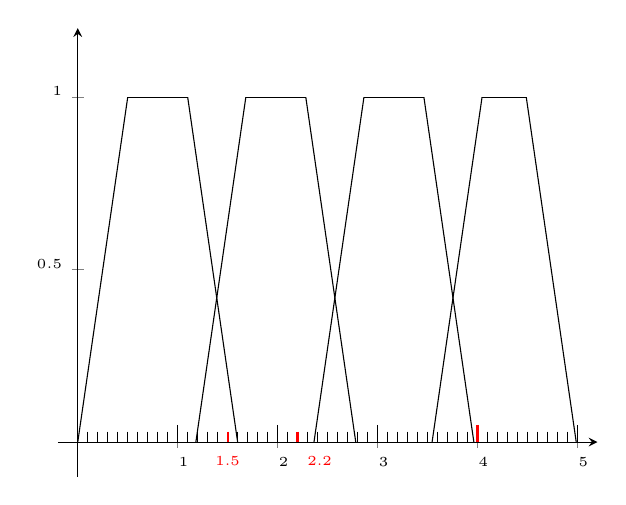
\begin{tikzpicture}[font=\tiny]
        \begin{axis} [
            xmin=-0.2, xmax=5.2, ymin=-0.1, ymax=1.2,
            % xlabel={$x$},
            xtick={0,1,...,5}, ytick={0,0.5,1},
            xticklabel style={font=\tiny, xshift=0.5ex},
            yticklabel style={font=\tiny, yshift=0.5ex},
            axis line style={->},
            axis x line=middle,
            axis y line=middle,
            % ticks=none,
            % grid=both,
          % legend pos=north west,
          % legend style={at={(0.05,0.8)},anchor=south west}
        ]

        \addplot+[mark=none,color=black, domain=0:0.5,solid] {2*x};
        \addplot+[mark=none,color=black,solid, domain=0.5:1.1] {1};
        \addplot+[mark=none,color=black,solid, domain=1.1:1.6] {-2*x+3.2};

        \addplot+[mark=none,color=black,solid, domain=0:0.5][xshift=1.5cm] {2*x};
        \addplot+[mark=none,color=black,solid, domain=0.5:1.1][xshift=1.5cm] {1};
        \addplot+[mark=none,color=black,solid, domain=1.1:1.6][xshift=1.5cm] {-2*x+3.2};


        \addplot+[mark=none,color=black,solid, domain=0:0.5][xshift=3cm] {x*2};
        \addplot+[mark=none,color=black,solid, domain=0.5:1.1][xshift=3cm] {1};
        \addplot+[mark=none,color=black,solid, domain=1.1:1.6][xshift=3cm] {-2*x+3.2};
        
        \addplot+[mark=none,color=black,solid, domain=0:0.5][xshift=4.5cm] {x*2};
        \addplot+[mark=none,color=black,solid, domain=0.5:0.95][xshift=4.5cm] {1};
        \addplot+[mark=none,color=black,solid, domain=1.1:1.6][xshift=4.3cm] {-2*x+3.2};        
        
        %%%%%%%%%%%%%%%%%%%%%%%%%%%%%%%%%%%%%%%%%%%%%%%%%%%%%%%%%%%%%%        
        \draw[] (0.1,0.03) -- (0.1,0);
        \draw[] (0.2,0.03) -- (0.2,0);
        \draw[] (0.3,0.03) -- (0.3,0);
        \draw[] (0.4,0.03) -- (0.4,0);
        \draw[] (0.5,0.03) -- (0.5,0);
        \draw[] (0.6,0.03) -- (0.6,0);
        \draw[] (0.7,0.03) -- (0.7,0);
        \draw[] (0.8,0.03) -- (0.8,0);
        \draw[] (0.9,0.03) -- (0.9,0);
        \draw[] (1.0,0.05) -- (1.0,0);
    
        \draw[] (1.1,0.03) -- (1.1,0);
        \draw[] (1.2,0.03) -- (1.2,0);        
        \draw[] (1.3,0.03) -- (1.3,0);
        \draw[] (1.4,0.03) -- (1.4,0);
        \draw[red,thick] (1.5,0.03) -- (1.5,0);
        \draw[] (1.6,0.03) -- (1.6,0);
        \draw[] (1.7,0.03) -- (1.7,0);
        \draw[] (1.8,0.03) -- (1.8,0);  
        \draw[] (1.9,0.03) -- (1.9,0);
        \draw[] (2.0,0.05) -- (2.0,0);        
        
        \draw[] (2.1,0.03) -- (2.1,0);
        \draw[red,thick] (2.2,0.03) -- (2.2,0);
        \draw[] (2.3,0.03) -- (2.3,0);
        \draw[] (2.4,0.03) -- (2.4,0);
        \draw[] (2.5,0.03) -- (2.5,0);
        \draw[] (2.6,0.03) -- (2.6,0);
        \draw[] (2.7,0.03) -- (2.7,0);
        \draw[] (2.8,0.03) -- (2.8,0);
        \draw[] (2.9,0.03) -- (2.9,0);
        \draw[] (3.0,0.05) -- (3.0,0);
    
        \draw[] (3.1,0.03) -- (3.1,0);
        \draw[] (3.2,0.03) -- (3.2,0);        
        \draw[] (3.3,0.03) -- (3.3,0);
        \draw[] (3.4,0.03) -- (3.4,0);
        \draw[] (3.5,0.03) -- (3.5,0);
        \draw[] (3.6,0.03) -- (3.6,0);
        \draw[] (3.7,0.03) -- (3.7,0);
        \draw[] (3.8,0.03) -- (3.8,0);  
        \draw[] (3.9,0.03) -- (3.9,0);
        \draw[red,thick] (4.0,0.05) -- (4.0,0);   


        \draw[] (4.1,0.03) -- (4.1,0);
        \draw[] (4.2,0.03) -- (4.2,0);
        \draw[] (4.3,0.03) -- (4.3,0);
        \draw[] (4.4,0.03) -- (4.4,0);
        \draw[] (4.5,0.03) -- (4.5,0);
        \draw[] (4.6,0.03) -- (4.6,0);
        \draw[] (4.7,0.03) -- (4.7,0);
        \draw[] (4.8,0.03) -- (4.8,0);
        \draw[] (4.9,0.03) -- (4.9,0);
        \draw[] (5.0,0.05) -- (5.0,0);

        \node[below, red] at (1.5,-0.015) {1.5};
        \node[below right,red] at (2.2,-0.015) {2.2};
        % \node[below] at (4.0,-0.015) {4.0};
        
        \end{axis}
   
\end{tikzpicture}
\end{document}

